\documentclass[table]{beamer}
%[]中可以使用draft、handout、screen、transparency、trancompress、compress等参数

%指定beamer的模式与主题
\mode<presentation>
{
  \usetheme{Madrid}
%\usetheme{Boadilla}
%\usecolortheme{default}
%\usecolortheme{orchid}
%\usecolortheme{whale}
%\usefonttheme{professionalfonts}
}

%\usetheme{Madrid}
%这里还可以选择别的主题:Bergen, Boadilla, Madrid, AnnArbor, CambridgeUS, Pittsburgh, Rochester, Warsaw, ...
%有导航栏的Antibes, JuanLesPins, Montpellier, ...
%有内容的Berkeley, PaloAlto, Goettingen, Marburg, Hannover, ...
%有最小导航栏的Berlin, Ilmenau, Dresden, Darmstadt, Frankfurt, Singapore, Szeged, ...
%有章和节表单的Copenhagen, Luebeck, Malmoe, Warsaw, ...

%\usecolortheme{default}
%设置内部颜色主题(这些主题一般改变block里的颜色);这个主题一般选择动物来命名
%这里还可以选择别的颜色主题,如默认的和有特别目的的颜色主题default,structure,sidebartab,全颜色主题albatross,beetle,crane,dove,fly,seagull,wolverine,beaver

%\usecolortheme{orchid}
%设置外部颜色主题(这些主题一般改变title里的颜色);这个主题一般选择植物来命名
%这里还可以选择别的颜色主题,如默认的和有特别目的的颜色主题lily,orchid,rose

%\usecolortheme{whale}
%设置字体主题;这个主题一般选择海洋动物来命名
%这里还可以选择别的颜色主题,如默认的和有特别目的的颜色主题whale,seahorse,dolphin

%\usefonttheme{professionalfonts}
%类似的还可以定义structurebold,structuresmallcapsserif,professionalfonts

% 控制 beamer 的风格,可以根据自己的爱好修改
%\usepackage{beamerthemesplit} %使用 split 风格
%\usepackage{beamerthemeshadow} %使用 shadow 风格
%\usepackage[width=2cm,dark,tab]{beamerthemesidebar}

%插入音标
%\usepackage{tipa}
%\AtBeginDocument{
  %\renewcommand\textipa{\fontencoding{T3}\selectfont}
%}
%\AtBeginDocument{
  %\renewcommand\textipa[2][r]{{\fontfamily{cm#1}\tipaencoding #2}}
%}
%\renewenvironment{IPA}[1][r]
 %{\fontfamily{cm#1}\tipaencoding}
 %{}

% 设定英文字体
%\usepackage{fontspec}
% Fix bugs for fontspec in TeXLive2015
\ifdefined\suppressfontnotfounderror
  \expandafter\let\csname xetex_suppressfontnotfounderror:D\endcsname
    \suppressfontnotfounderror
\else
  \expandafter\let\csname xetex_suppressfontnotfounderror:D\endcsname
    \luatexsuppressfontnotfounderror
\fi
\usepackage[no-math]{fontspec}
\setmainfont{Times New Roman}
\setsansfont{Arial}
\setmonofont{Courier New}

% 设定中文字体
\usepackage[BoldFont,SlantFont,CJKchecksingle,CJKnumber]{xeCJK}
%\setCJKmainfont[BoldFont={Adobe Heiti Std},ItalicFont={Adobe Kaiti Std}]{Adobe Song Std}
\setCJKmainfont[BoldFont={Adobe Heiti Std},ItalicFont={Adobe Kaiti Std}]{WenQuanYi Micro Hei}
\setCJKsansfont{Adobe Heiti Std}
\setCJKmonofont{Adobe Fangsong Std}
\punctstyle{hangmobanjiao}

\defaultfontfeatures{Mapping=tex-text}
\usepackage{xunicode}
\usepackage{xltxtra}

\XeTeXlinebreaklocale "zh"
\XeTeXlinebreakskip = 0pt plus 1pt minus 0.1pt

\usepackage{setspace}
\usepackage{colortbl,xcolor}
\usepackage{hyperref}
%\hypersetup{xetex,bookmarksnumbered=true,bookmarksopen=true,pdfborder=1,breaklinks,colorlinks,linkcolor=blue,filecolor=black,urlcolor=cyan,citecolor=green}
\hypersetup{xetex,bookmarksnumbered=true,bookmarksopen=true,pdfborder=1,breaklinks,colorlinks,linkcolor=cyan,filecolor=black,urlcolor=blue,citecolor=green}

% 插入图片
\usepackage{graphicx}
\graphicspath{{figures/}}
% 图文混排
%\usepackage{picins}
\usepackage{floatflt}

% 可能用到的包
\usepackage{amsmath,amssymb}
%插入多媒体
%\usepackage{media9}
%\usepackage{movie15}
\usepackage{multimedia}
\usepackage{multicol}
\usepackage{multirow}

% 定义一些自选的模板,包括背景、图标、导航条和页脚等,修改要慎重
% 设置背景渐变由10%的红变成10%的结构颜色
%\beamertemplateshadingbackground{red!10}{structure!10}
%\beamertemplatesolidbackgroundcolor{white!90!blue}
% 使所有隐藏的文本完全透明、动态,而且动态的范围很小
\beamertemplatetransparentcovereddynamic
% 使itemize环境中变成小球,这是一种视觉效果
\beamertemplateballitem
% 为所有已编号的部分设置一个章节目录,并且编号显示成小球
\beamertemplatenumberedballsectiontoc
% 将每一页的要素的要素名设成加粗字体
\beamertemplateboldpartpage

% item逐步显示时,使已经出现的item、正在显示的item、将要出现的item呈现不同颜色
\def\hilite<#1>{
 \temporal<#1>{\color{gray}}{\color{blue}}
    {\color{blue!25}}
}

\renewcommand{\today}{\number\year 年 \number\month 月 \number\day 日}

%五角星
\usepackage{MnSymbol}

%去除图表标题中的figure等
\usepackage{caption}
\captionsetup{labelformat=empty,labelsep=none}

\usepackage{tabu}
\usepackage{multirow}
%表格自动换行
\usepackage{tabularx} 

% 千分号
%\usepackage{textcomp}

%罗马数字
\makeatletter
\newcommand{\rmnum}[1]{\romannumeral #1}
\newcommand{\Rmnum}[1]{\expandafter\@slowromancap\romannumeral #1@}
\makeatother

%分栏
\usepackage{multicol}

%\usepackage{enumitem}
%\usepackage{enumerate}

%键盘
\usepackage{keystroke}

%心形
\usepackage{fdsymbol}

%插入源代码
\usepackage{listings}
\lstset{
  language=perl,                  % 程序语言名称:TeX, Perl, R, sh, bash, Awk
  basicstyle=\normalsize\tt,      %\tt指monospace字体族,程序源代码使用此族字体表示更加美观
  numbers=left,                   % 行号位置(左侧)
  numberstyle=\small,             % 行号字体的字号
  stepnumber=1,                   % 行号的显示步长
  numbersep=5pt,                  % 行号与代码间距
  backgroundcolor=\color{white},  % 背景色;需要 \usepackage{color}
  showspaces=false,               % 不显示空格
  showstringspaces=false,         % 不显示代码字符串中的空格标记
  showtabs=false,                 % 不显示 TAB
  tabsize=4, 
  frame=shadowbox,                % 把代码用带有阴影的框圈起来
  captionpos=b,                   % 标题位置
  breaklines=true,                % 对过长的代码自动断行
  breakatwhitespace=false,        % 断行只在空格处
  extendedchars=false,            % 解决代码跨页时,章节标题,页眉等汉字不显示的问题
  %escapeinside={\%*}{*},         % 跳脱字符,添加注释,暂时离开 listings 
  %escapeinside=``,
  commentstyle=\color{red!50!green!50!blue!50}\tt,  %浅灰色的注释
  rulesepcolor=\color{red!20!green!20!blue!20},     %代码块边框为淡青色
  keywordstyle=\color{blue!70}\bfseries\tt,         %代码关键字的颜色为蓝色,粗体
  identifierstyle=\tt,
  stringstyle=\tt,                % 代码字符串的特殊格式
  keepspaces=true,
  breakindent=1em,
  %breakindent=22pt,
  %breakindent=4em,
  breakautoindent=true,
  flexiblecolumns=true,
  aboveskip=1em,                  %代码块边框
  xleftmargin=2em,
  xrightmargin=2em
}

%\setbeamercolor{alerted text}{fg=magenta}
\setbeamercolor{bgcolor}{fg=yellow,bg=cyan}
%\setbeamercolor{itemize/enumerate body}{fg=green}

\begin{document}

%\includeonlyframes{current}

\logo{\includegraphics[height=0.08\textwidth]{tijmu.png}}

% 在每个Section前都会加入的Frame
\AtBeginSection[]
{
  \begin{frame}<beamer>
    %\frametitle{Outline}
    \frametitle{教学提纲}
    \setcounter{tocdepth}{3}
    \begin{multicols}{2}
      \tableofcontents[currentsection,currentsubsection]
      %\tableofcontents[currentsection]
    \end{multicols}
  \end{frame}
}
% 在每个Subsection前都会加入的Frame
\AtBeginSubsection[]
{
  \begin{frame}<beamer>
%%\begin{frame}<handout:0>
%% handout:0 表示只在手稿中出现
    \frametitle{教学提纲}
    \setcounter{tocdepth}{3}
    \begin{multicols}{2}
    \tableofcontents[currentsection,currentsubsection]
    \end{multicols}
%% 显示在目录中加亮的当前章节
  \end{frame}
}

% 为当前幻灯片设置背景
%{
%\usebackgroundtemplate{
%\vbox to \paperheight{\vfil\hbox to
%\paperwidth{\hfil\includegraphics[width=2in]{tijmu_charcoal.png}\hfil}\vfil}
%}
\begin{frame}[plain]
  \begin{center}
    {\Huge 分子生物计算\\}
    {\huge \textit{(Perl语言编程)}\\}
    \vspace{1cm}
    {\LARGE 天津医科大学\\}
    %\vspace{0.2cm}
    {\LARGE 生物医学工程与技术学院\\}
    \vspace{1cm}
    {\large 2019-2020学年上学期(秋)\\ 2017级生信班}
  \end{center}
\end{frame}
%}



\title[TIMTOWTDI]{TIMTOWTDI\\(条条大路通罗马)}
\author[Yixf]{伊现富(Yi Xianfu)}
\institute[TIJMU]{天津医科大学(TIJMU)\\ 生物医学工程与技术学院}
\date{2019年1月}

%\input{snippet/beamer_toc.tex}
\begin{frame}
  \titlepage
\end{frame}

\begin{frame}[fragile]
  \frametitle{帮助文档}
  \vspace{-1.5em}
\begin{lstlisting}
# The Perl 5 language interpreter
man perl
# Look up Perl documentation in Pod format
man perldoc
perldoc perldoc

# Perl built-in function
perldoc -f BuiltinFunction
perldoc -f substr
# FAQ
perldoc -q FAQKeyword
perldoc -q random
# Perl predefined variable
perldoc -v PerlVariable
perldoc -v '$_'
\end{lstlisting}
\end{frame}

\begin{frame}[fragile]
  \frametitle{启用警告}
  \vspace{-1.5em}
\begin{lstlisting}
# Method1
# 使用命令行选项-w
perl -w script.pl

# Method2
# 在命令解释行使用-w
#!/usr/bin/perl -w

# Method3
# 使用use
use warnings;
\end{lstlisting}
\end{frame}

\begin{frame}[fragile]
  \frametitle{字符串拼接}
  \vspace{-1.5em}
\begin{lstlisting}
# Method1
$DNA3 = "$DNA1$DNA2"; print "$DNA3\n";

# Method2
print "$DNA1$DNA2\n";

# Method3
print $DNA1, $DNA2, "\n";

# Method4
$DNA3 = $DNA1 . $DNA2; print "$DNA3\n";

# Method5
$DNA3 = join "", $DNA1, $DNA2; print "$DNA3\n";
\end{lstlisting}
\end{frame}

\begin{frame}[fragile]
  \frametitle{文件读取}
  \vspace{-1.5em}
\begin{lstlisting}
# Method1(只读取一行)
$protein = <PROTEINFILE>;

# Method2(读取所有行,一次性保存进数组)
@proteins = <PROTEINFILE>;

# Method3(依次读取每一行)
while (<PROTEINFILE>) {
  ...actions...
}

# Method4(读取所有行,一次性保存进标量)
$protein = do { local $/; <PROTEINFILE>; };
\end{lstlisting}
\end{frame}

\begin{frame}[fragile]
  \frametitle{获取数组元素个数}
  \vspace{-1.5em}
\begin{lstlisting}
# Methods1
$num = scalar @bases;

# Methods2
$num = @bases;

#Methods3
$num = $#bases + 1;
\end{lstlisting}
\end{frame}

\begin{frame}[fragile]
  \frametitle{获取数组的第一个元素}
  \vspace{-1.5em}
\begin{lstlisting}
# Method1
$first_gene = $genes[0];
#($first_gene) = $genes[0];

# Method2
($first_gene) = @genes;

# Method3
$first_gene = shift @genes;
# 注意:shift会影响原始的@genes数组
\end{lstlisting}
\end{frame}

\begin{frame}[fragile]
  \frametitle{获取数组的最后一个元素}
  \vspace{-1.5em}
\begin{lstlisting}
# Method1
$last_gene = $genes[-1];

# Method2
$last_gene = $genes[$#genes];

# Method3
$last_gene = pop @genes;
# 注意:pop会影响原始的@genes数组
\end{lstlisting}
\end{frame}

\begin{frame}[fragile]
  \frametitle{变量值+1}
  \vspace{-1.5em}
\begin{lstlisting}
# Methods1
$count++;

# Methods2
++$count;

# Methods3
$count += 1;

# Methods4
$count = $count + 1;
\end{lstlisting}
\end{frame}

\begin{frame}[fragile]
  \frametitle{计数核苷酸}
  \vspace{-1.5em}
\begin{lstlisting}
# Methods1(使用数组)
@DNA = split( '', $DNA );
foreach $base (@DNA) { ...count... }
# Methods2(操作字符串)
for ( $pos=0 ; $pos < length $DNA ; ++$pos ) {
  $base = substr( $DNA, $pos, 1 ); ..count..
}
# Methods3(模式匹配)
while ( $DNA =~ /a/ig ) { $a++ }
while ( $DNA =~ /[^acgt]/ig ) { $e++ }
# Methods4(使用tr函数)
$a = ($DNA =~ tr/Aa/Aa/);
$basecount = ($DNA =~ tr/ACGTacgt/ACGTacgt/);
$nonbase = (length $DNA) - $basecount;
\end{lstlisting}
\end{frame}

\begin{frame}[plain]
\end{frame}

\begin{frame}
  \frametitle{考试}
  \begin{block}{考试安排}
    \begin{itemize}
      \item 时间:1.9(周一),10:30-12:10
      \item 地点:西楼510
      \item 时长:100分钟
      \item 总分:100分
    \end{itemize}
  \end{block}
  \pause
  \begin{block}{题型与分值}
    \begin{enumerate}
      \item 单选题:$25 \times 1  = 25$
      \item 多选题:$20 \times 1  = 20$
      \item 简答题:$4  \times 5  = 20$
      \item 编程题:$5  \times 5  = 25$
      \item 应用题:$1  \times 10 = 10$
    \end{enumerate}
  \end{block}
\end{frame}

\begin{frame}
  \frametitle{知识点}
  \begin{itemize}
    \item 生物学基础:拉丁语,数据库,碱基/氨基酸代码,限制酶,点突变
    \item R:常用包
    \item Markdown:基本语法,格式转换
    \item Git:基本使用
    \item Perl基础:CPAN,变量,赋值,use *,三大数据类型,上下文,子程序,调试器,排序,命令行参数,随机,关系数据库,my,编程流程,特殊变量,编程策略,构思步骤,字符串拼接,文件读取写入,perldoc,模块,设计理念,流程控制
    \item 数组:索引,操作,split,join
    \item 测试:条件操作符,字符串/数字/文件测试,真假
    \item 正则表达式:元字符,修饰符,匹配,替换,tr
    \item 编程:DNA突变,相似性计算,限制酶的正则表征,子程序传递,序列两两比较,阅读框翻译,……
  \end{itemize}
\end{frame}

\begin{frame}
  \frametitle{FATSQ}
  \begin{figure}
    \centering
    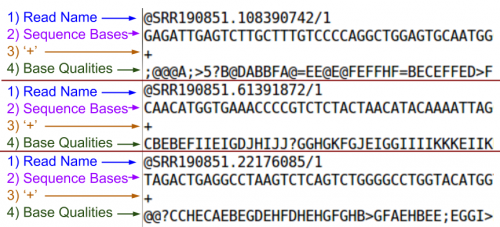
\includegraphics[width=0.35\textwidth]{fastq_01.png}
    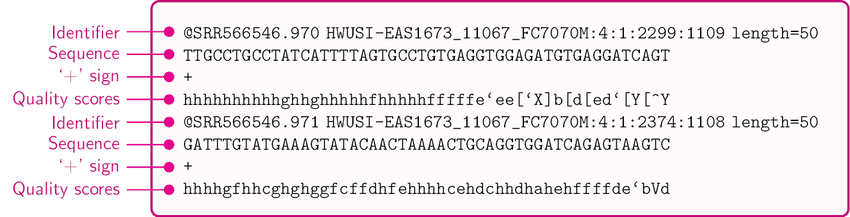
\includegraphics[width=0.6\textwidth]{fastq_04.png}\\
    \vspace{1em}
    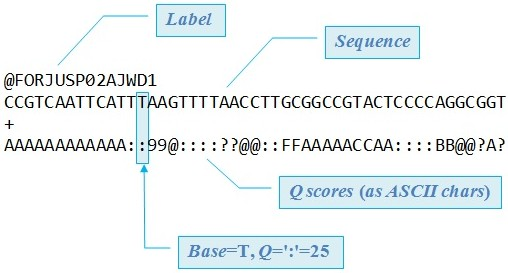
\includegraphics[width=0.35\textwidth]{fastq_03.jpg}
    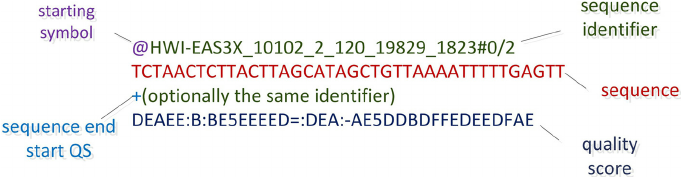
\includegraphics[width=0.6\textwidth]{fastq_02.png}\\
    \vspace{1em}
    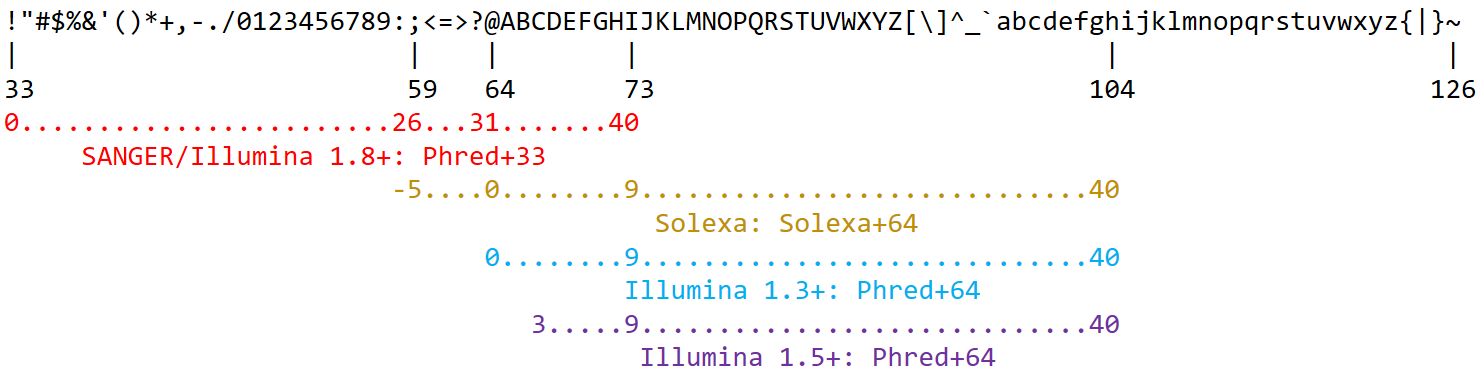
\includegraphics[width=0.9\textwidth]{fastq_05.png}
  \end{figure}
\end{frame}

\input{snippet/class_tail.tex}
